
\subsection{Epoch Analysis}
Wavelet analysis of the NAM and AMOC indices suggests that within the 1000 year simulation, intervals of distinct, periodic, co-varying behaviour occurs between the two modes. To examine the nature of these different interactions individually we split the simulation into epochs and analyse the association between the stratosphere and the ocean in each. 

We define epoch 1 to span year numbers xxx-xxx which covers the interval in which significant cross power is found at 90-100 year periods between the AMOC at 45N and the filtered NAM index (see figure \ref{NAM_AMOC_Cross}). Composites of AMOC behaviour around extreme events in this epoch (figure \ref{epoch_composites_combined} are characterised by two prominent features: Negative anomalies in the AMOC at a lag of 10-20 years after events and positive anomalies preceding events by approximately 20-25 years. The AMOC pattern within this epoch is consistent with 90-100 variability as the peak and trough of AMOC behaviour appear approximately 40-45 years apart which corresponds to half a 90 year cycle. The phase relationship suggested by the cross spectrum is also evident in the composite with peaks in the NAM leading troughs in the AMOC by a quarter of a cycle or positive peaks in the NAM leading positive NAM anomalies also by a quarter cycle. Deep Ocean temperature anomalies over the Labrador sea about events (figure \ref{epoch_composites_combined}g) exhibit large positive anomalies preceding the negative response in the AMOC to the NAM. Similar to patterns over the whole simulation (figure xxxx) these temperature anomalies at shallow depths (0-100m) and propagate downwards with time.

Epoch 2, which encompasses year numbers xxx-xxx, accounts for the portion of the cross spectra that exhibited significant power at the 30 year period timescale. In this epoch, only strong persistent vortex events are observed so we include the composite AMOC around only these types of events as opposed to the difference between strong and weak events in other epochs. This epoch shows positive AMOC anomalies at a lag of approximately 3 years after NAM events. This result reflects the phase relationship indicated by arrows on the cross spectra of figure \ref{NAM_AMOC_Cross} - a shift of a small portion of a cycle with the NAM leading. In addition, negative AMOC anomalies at a lag of 15-20 years are also visible, this feature is the same as in epoch 1. There are also negative AMOC anomalies preceding events by approximately 10 years and this set of 3 anomalies is consistent with 30 year timescale behaviour as successive peaks in the AMOC are approximately 30 years apart. Despite the fact that only strong event composites are included in this epoch, the magnitude of responses are still large and comparable to other epochs which show composite differences. A possible explanation of this is that this epoch includes the 2 largest values of the filtered NAM found in year number 349 and 376. This may inflate the magnitude of response patterns in this epoch. Similarly to epoch 1, the negative AMOC response at 15-20 year lags is associated with deep ocean temperature anomalies originating approximately 10 years after events and propagating downwards with time while increasing in magnitude until around 15 years after NAM events. 

\begin{center}
\begin{figure}[h!]
\noindent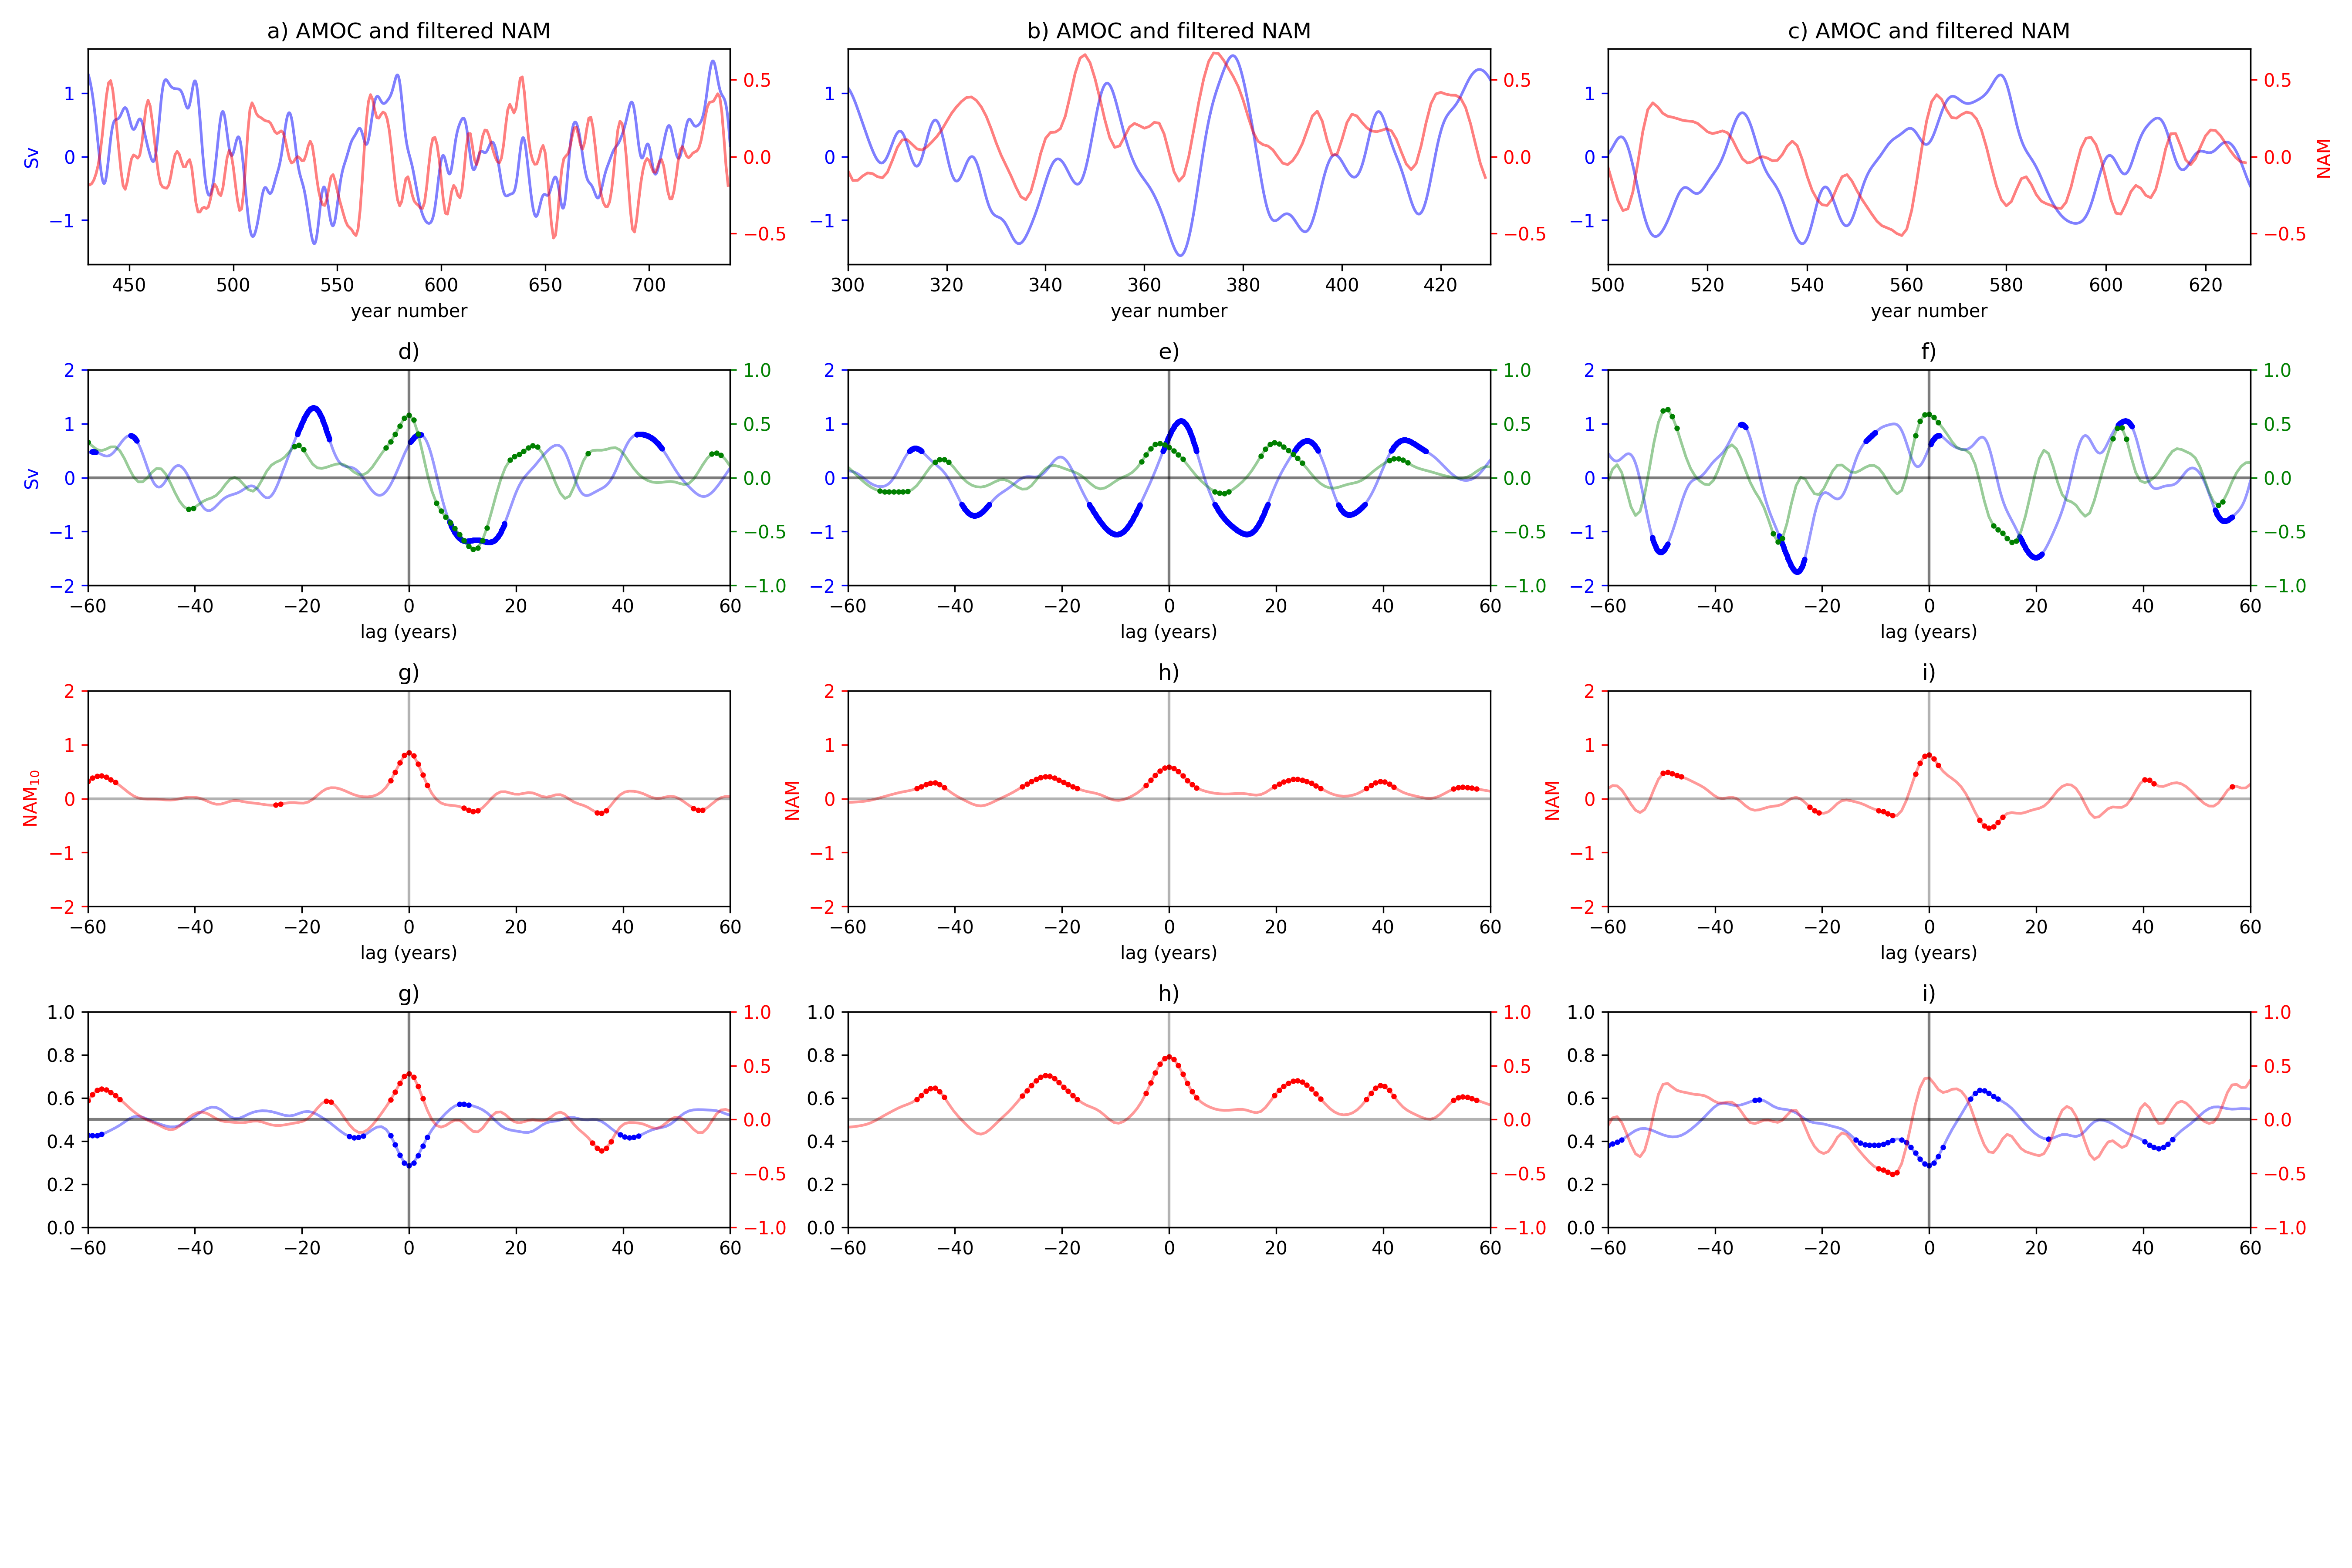
\includegraphics[width =\linewidth]{figures/AMOC_deep_T_combined.png}
\caption{Characteristics of variability in epoch 1 (a,d,g), epoch 2 (b,e,h) and epoch 3 (c,f,i) of the UKESM simulation. a-c: filtered Dec-Mar NAM and AMOC at 45N. d-f: Lagged response of AMOC index at 45N to persistent NAM events. Blue series shows AMOC composite difference values between positive and negative NAM events. The $x$ axis denotes the lead (negative values) or lag (positive values) relative to the event date. Black dots denote composited differences under a two tailed student's t-test. In all cases the AMOC values have been seasonally detrended by removing the seasonal cycle.
g-i: deep ocean temperature anomaly associated with persistent NAM events. Shading shows temperature values and only anomalies significant under a 2 tailed student's t-test are included.}
\label{epoch_composites_combined}
\end{figure}
\end{center}

%Epoch 3 is characterised by 50 year period variability in both modes (year numbers xxx-xxx) and exhibits two negative anomalies in the AMOC 30 years preceding and 20-25 years following NAM events respectively. There are also small significant anomalies at lags of approximately 3 years consistent with the phases relationship indicated on cross spectrum in this epoch (NAM leading by a small portion of the cycle). One would expect larger anomalies at these short lags in this epoch due to the 50 year variations present, however The lack of prominent positive anomaly may be due to the fact that epoch 3 coincides with epoch 1 in which minimal anomalies are observed at these lags. As a result, we expect the pattern in epoch 3 to represent a superposition of signals from both epochs which may lead to a damping of the response at lakgs of around 3 years. Once again, negative anomalies at lags of $\sim$20 years are associated with descending positive signals in Labrador seas deep ocean temperatures. 

%These results show that AMOC patterns associated with NAM extremes are different across epochs depending on the dominant periods of variability present. As a result, composites such as those shown in figures \ref{AMOC_comp_NAM} and \ref{AMOC_comp_NAM_lowpass} may arise from a superposition of patterns from different timescales of variability. However, while AMOC patterns are different across epochs, one element of behaviour is constant: Negative anomalies in the AMOC $\sim$20 years following persistent NAM events associated with positive, deep anomalies in Labrador Sea ocean temperatures. This may suggest the presence of a single underlying coupling mechanism between the two modes which modulates the AMOC patterns associated with events in different epochs. As such, the differing phase relationships across epochs arise from this modulation with anomalies at different leads/lags set by the position 20 year lag response as well as the length of the cycles involved in a given epoch. For example, in epoch 2 the positive anomaly at 3 year lag as well as the negative anomaly at 10 years preceding the NAM are present because they appear approximately 15 years (1/2 a cycle) and 30 years (1 cycle) before the 20 year lag response. The phase relationship on the cross spectrum subsequently identifies the 3 year lagged response despite the 20 year lag anomaly holding responsibility for physical coupling. In the following sections, we examine this 20 year lagged response more closely and analyse possible physical pathways involved in the coupling between the vortex and the AMOC.


